\section{The Need for Time-to-Event Analysis}

Many real-world scenarios require us to understand not just \textit{if} an event will occur, but \textit{when} it might happen. This timing aspect adds complexity to traditional predictive modeling approaches, but also provides valuable information that can lead to better decision-making and outcomes.

\begin{notebox}[title=Time-to-Event Questions Across Domains]
  Time-to-event analysis answers crucial questions across numerous fields:
  \begin{itemize}
  \item \textbf{Healthcare:} When will a patient experience disease progression? How long will a treatment remain effective?
  \item \textbf{Engineering:} How long will a mechanical component function before failure? When should maintenance be scheduled?
  \item \textbf{Business:} When will a customer likely cancel their subscription? When might an employee leave the company?
  \item \textbf{Technology:} When will a system failure occur? What is the expected lifetime of a software feature?
  \end{itemize}
\end{notebox}

Traditional predictive models typically focus on classification (will an event occur?) or regression (how much of something will occur?), but time-to-event analysis introduces a temporal dimension that requires specialized methodologies. Without proper handling of the time component, predictions can be severely biased and lead to incorrect conclusions.

\section{Applications Across Domains}

The need for time-to-event analysis spans virtually every field where timing information is critical for decision-making.

\subsection{Healthcare Applications}

In medicine, understanding the timing of events can directly impact treatment decisions and patient outcomes:

\begin{itemize}
\item \textbf{Patient survival analysis:} Estimating survival time after diagnosis or treatment
\item \textbf{Disease progression:} Predicting time to progression or recurrence
\item \textbf{Treatment efficacy:} Determining duration of treatment effectiveness
\item \textbf{Adverse event timing:} Analyzing when side effects might occur
\item \textbf{Hospital readmission:} Predicting when patients might return after discharge
\item \textbf{Clinical trial analysis:} Comparing time-to-event outcomes between treatment groups
\end{itemize}

Time-to-event analysis in healthcare directly informs treatment planning, resource allocation, and the development of clinical guidelines.

\subsection{Engineering and Reliability Applications}

In engineering contexts, time-to-event analysis helps optimize maintenance schedules, warranty periods, and resource allocation:

\begin{itemize}
\item \textbf{Equipment failure prediction:} Estimating when machinery might fail
\item \textbf{Component lifetime estimation:} Predicting the functional lifespan of parts
\item \textbf{Maintenance optimization:} Scheduling preventive maintenance to minimize downtime
\item \textbf{System reliability assessment:} Evaluating the reliability of complex systems over time
\item \textbf{Warranty period modeling:} Setting appropriate warranty terms based on failure timing
\item \textbf{Quality control:} Analyzing time-to-failure patterns to improve manufacturing
\end{itemize}

These applications help reduce costs, improve safety, and enhance product quality.

\subsection{Business and Economic Applications}

In business contexts, time-to-event analysis provides insights into customer behavior, employee retention, and financial risk:

\begin{itemize}
\item \textbf{Customer churn prediction:} Forecasting when customers might leave
\item \textbf{Subscription lifecycle:} Modeling subscription duration patterns
\item \textbf{Employee retention:} Predicting when employees might leave
\item \textbf{Loan default timing:} Estimating when borrowers might default
\item \textbf{Insurance claim occurrence:} Predicting timing of insurance claims
\item \textbf{Project completion:} Modeling time-to-completion for projects
\end{itemize}

These applications help businesses optimize resource allocation, improve customer retention strategies, and manage financial risk.

\subsection{Other Diverse Applications}

Time-to-event analysis extends to many other fields:

\begin{itemize}
\item \textbf{Social sciences:} Modeling unemployment duration, marriage longevity
\item \textbf{Technology:} Predicting software bug discovery rates, digital content lifespan
\item \textbf{Environmental science:} Analyzing timing of extreme events, species extinction risks
\item \textbf{Academia:} Studying citation timing, research impact evolution
\item \textbf{Public policy:} Evaluating time-dependent effects of policy interventions
\end{itemize}

The ubiquity of time-to-event questions across domains highlights the critical importance of developing robust methodologies for modeling and analyzing such data.

\section{Unique Characteristics of Time-to-Event Data}

Time-to-event data presents several distinct challenges that require specialized analytical approaches. These characteristics make standard regression or classification methods inadequate without careful modification.

\subsection{Incomplete Observations}

Unlike conventional datasets where each observation has a complete set of values, time-to-event data frequently includes incomplete observations—a phenomenon known as censoring. Censoring occurs when the event of interest is not observed for some subjects, but we still have partial information about their event times.

In a clinical study, for example, patients may:
\begin{itemize}
\item Still be alive at the end of the study period
\item Withdraw from the study before experiencing the event
\item Be lost to follow-up for various reasons
\end{itemize}

These incomplete observations contain valuable information that must be properly incorporated into the analysis rather than discarded.

\subsection{Variable Follow-up Durations}

Subject follow-up periods typically vary considerably within a single dataset, with some subjects observed for short periods and others for much longer. This variability creates challenges for standardizing predictions and assessing model performance.

\subsection{Time-Varying Covariates}

Many predictors in time-to-event contexts change over the observation period. For example:
\begin{itemize}
\item A patient's biomarker values may fluctuate during treatment
\item A machine's operational parameters may shift over time
\item A customer's engagement metrics may evolve throughout the relationship
\end{itemize}

These dynamic covariates need special handling to accurately model their effects on the timing of events.

\subsection{Multiple Competing Events}

In many real-world scenarios, subjects may experience various mutually exclusive events:
\begin{itemize}
\item A patient might die from cancer, heart disease, or other causes
\item A mechanical system might fail due to wear, electrical issues, or external damage
\item A customer might churn for different reasons (price, service quality, competitor offers)
\end{itemize}

These competing events require models that can account for multiple possible outcomes and their interdependencies.

\subsection{Informative Observation Patterns}

In time-to-event data, the pattern of observations itself may contain information relevant to the outcome. For example, the frequency of patient visits might correlate with disease severity, or the timing of system inspections might relate to suspected issues. This informative missingness adds another layer of complexity to the analysis.

\section{The Fundamental Challenge: Censoring}

Censoring—the partial observation of event times—represents the most distinctive and challenging aspect of time-to-event data. Censoring occurs when we don't observe the exact time of the event for a subject, but we have some information about when it might have occurred.

A comprehensive discussion of censoring types, mechanisms, and their implications can be found in Chapter \ref{ch:censoring}. Here, we highlight the key challenges that censoring introduces in time-to-event analysis.

\begin{notebox}[title=Key Challenges with Censored Data]
Censoring introduces several unique challenges:
\begin{itemize}
\item Standard statistical methods cannot be directly applied
\item Naive approaches (ignoring censored observations or treating censoring times as event times) lead to biased results
\item Different forms of censoring require different analytical approaches
\item Assumptions about the censoring mechanism are critical for valid inference
\end{itemize}
\end{notebox}

\section{Visualizing Survival Data}

A comprehensive visual representation of survival data helps illustrate the unique challenges of time-to-event analysis. Figure \ref{fig:survival-data-viz} shows a typical survival dataset with varying follow-up times and both observed events and censored observations.

\begin{figure}[htbp]
  \centering
  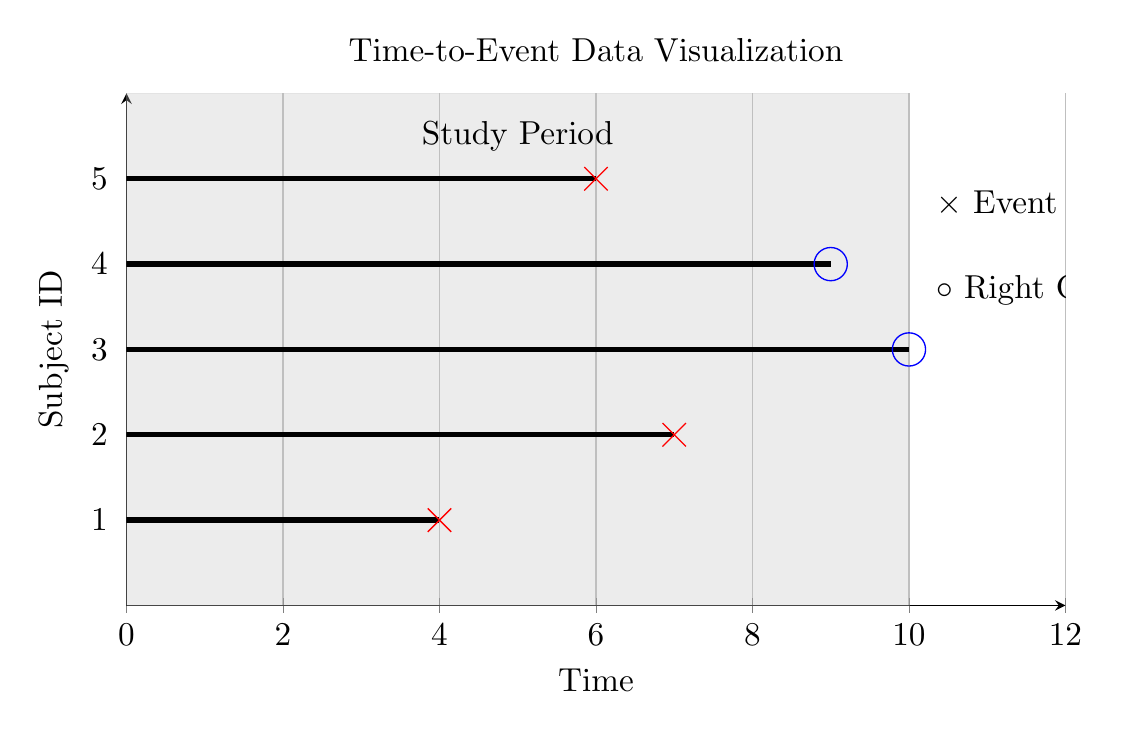
\begin{tikzpicture}[scale=1.2]
    \begin{axis}[
        width=0.95\textwidth,
        height=7cm,
        xlabel={Time},
        ylabel={Subject ID},
        axis lines=left,
        ymin=0,
        ymax=6,
        xmin=0,
        xmax=12,
        ytick={1,2,3,4,5},
        ytick style={draw=none},
        xmajorgrids=true,
        title={Time-to-Event Data Visualization},
      ]
      % Study period
      \addplot[color=lightgray, fill=lightgray, opacity=0.3] coordinates {
        (0,0) (0,6) (10,6) (10,0)
      } \closedcycle;
      \node at (axis cs:5,5.5) {Study Period};

      % Subject follow-up lines
      \addplot[ultra thick, -] coordinates {(0,1) (4,1)};
      \addplot[ultra thick, -] coordinates {(0,2) (7,2)};
      \addplot[ultra thick, -] coordinates {(0,3) (10,3)};
      \addplot[ultra thick, -] coordinates {(0,4) (9,4)};
      \addplot[ultra thick, -] coordinates {(0,5) (6,5)};

      % Events
      \addplot[mark=x, color=red, mark size=5pt] coordinates {(4,1)};
      \addplot[mark=x, color=red, mark size=5pt] coordinates {(7,2)};
      \addplot[mark=o, color=blue, mark size=5pt] coordinates {(10,3)};
      \addplot[mark=o, color=blue, mark size=5pt] coordinates {(9,4)};
      \addplot[mark=x, color=red, mark size=5pt] coordinates {(6,5)};

      % Legend
      \node[anchor=north west] at (axis cs:10.2,5) {$\times$ Event Observed};
      \node[anchor=north west] at (axis cs:10.2,4) {$\circ$ Right Censored};
    \end{axis}
  \end{tikzpicture}
  \caption{Visualization of time-to-event data for five subjects. Each horizontal line represents a subject's follow-up period. Red crosses indicate observed events, while blue circles represent right-censored observations. Note the varying follow-up durations and the mixture of event types.}
  \label{fig:survival-data-viz}
\end{figure}

This visualization highlights several key characteristics of survival data:

\begin{itemize}
\item \textbf{Variable follow-up durations:} Subjects are observed for different periods
\item \textbf{Mixture of observed events and censoring:} Some subjects experience the event during observation, while others are censored
\item \textbf{Administrative censoring:} Some subjects are censored at the study end
\item \textbf{Early withdrawals:} Some subjects exit the study before its conclusion
\end{itemize}

\section{Competing Risks: Another Challenge}

Another significant challenge in time-to-event analysis is the presence of competing risks—multiple possible event types where the occurrence of one event precludes the observation of others. Chapter \ref{ch:censoring} provides a detailed discussion of competing risks, their analysis, and modeling approaches.

Competing risks fundamentally change how we approach survival analysis:

\begin{itemize}
\item \textbf{Event-specific hazards:} Each event type has its own hazard function
\item \textbf{Cumulative incidence functions:} Standard Kaplan-Meier estimates become inappropriate; we need to use cumulative incidence functions that account for competing events
\item \textbf{Interpretation changes:} Risk factors may have different effects on different event types
\item \textbf{Modeling complexity:} Models must account for the interdependence between different event types
\end{itemize}

Ignoring competing risks can lead to substantial biases, particularly the overestimation of event probabilities when using standard survival methods.

\section{Beyond Binary Events: Complex Time-to-Event Scenarios}

Real-world time-to-event scenarios often extend beyond simple binary events (occurred/not occurred) to include more complex patterns:

\subsection{Recurrent Events}

Many events can occur multiple times for the same subject:

\begin{itemize}
\item Hospital readmissions
\item Equipment failures and repairs
\item Episodic disease flares
\item Repeated customer purchases
\end{itemize}

Recurrent event analysis requires specialized methods that can model the correlation between events within the same subject and account for potential changes in risk patterns after each event.

\subsection{Multi-State Processes}

In multi-state processes, subjects can transition through various states over time:

\begin{itemize}
\item Disease progression through different stages
\item Employee transitions between roles
\item Customer journey through different product tiers
\item System transitions between operational states
\end{itemize}

Multi-state models extend survival analysis to handle these complex transition patterns, with each transition potentially having its own risk factors and temporal patterns.

\begin{figure}[htbp]
  \centering
  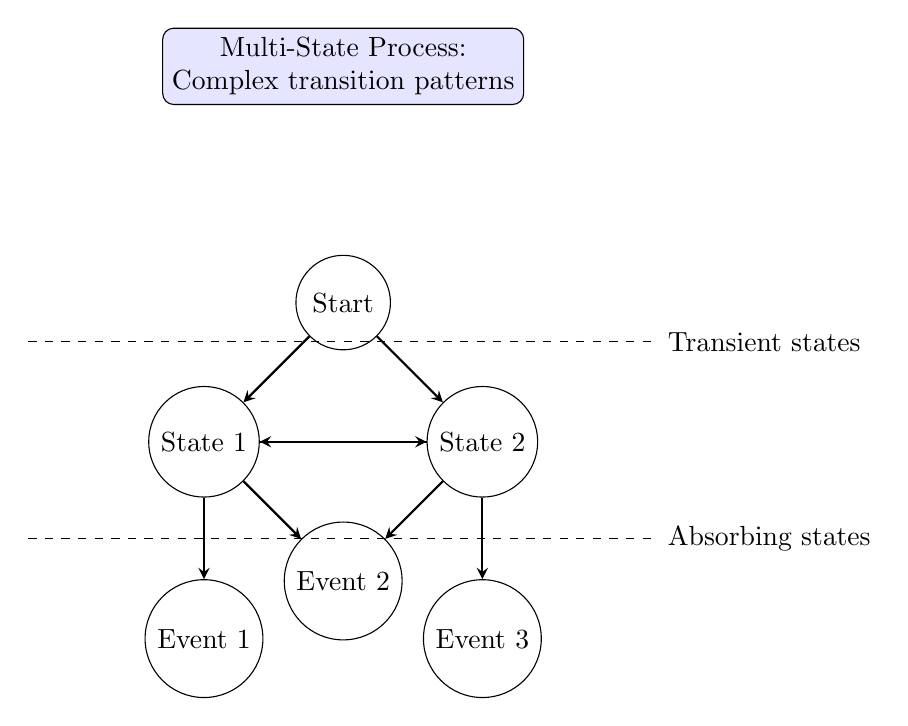
\begin{tikzpicture}[
      node distance=2.5cm,
      state/.style={circle, draw, minimum size=1.2cm},
      arrow/.style={->, >=stealth, thick}
    ]
    % States
    \node[state] (start) {Start};
    \node[state, below left of=start] (state1) {State 1};
    \node[state, below right of=start] (state2) {State 2};
    \node[state, below of=state1] (event1) {Event 1};
    \node[state, below of=state2] (event3) {Event 3};
    \node[state, below right of=state1] (event2) {Event 2};

    % Transitions
    \draw[arrow] (start) -- (state1);
    \draw[arrow] (start) -- (state2);
    \draw[arrow] (state1) -- (state2);
    \draw[arrow] (state2) -- (state1);
    \draw[arrow] (state1) -- (event1);
    \draw[arrow] (state1) -- (event2);
    \draw[arrow] (state2) -- (event2);
    \draw[arrow] (state2) -- (event3);

    % Annotations
    \node[draw, rounded corners, fill=blue!10, align=center] at (0,3) {
      Multi-State Process:\\
      Complex transition patterns
    };
    \draw[dashed] (-4,-0.5) -- (4,-0.5) node[right] {Transient states};
    \draw[dashed] (-4,-3) -- (4,-3) node[right] {Absorbing states};
  \end{tikzpicture}
  \caption{A multi-state process model. Subjects can transition between transient states and eventually reach absorbing states (terminal events). Each transition has its own hazard function that may depend on subject characteristics and history.}
  \label{fig:multi-state}
\end{figure}

\subsection{Joint Longitudinal and Time-to-Event Data}

In many applications, we observe both:
\begin{itemize}
\item Longitudinal measurements of variables over time (e.g., biomarkers, system parameters)
\item Time-to-event outcomes (e.g., failure, disease progression)
\end{itemize}

Joint models for longitudinal and time-to-event data enable:
\begin{itemize}
\item Incorporating time-varying measurements into event predictions
\item Accounting for measurement error in longitudinal data
\item Addressing informative dropout in longitudinal studies
\item Providing dynamic, updated predictions as new measurements arrive
\end{itemize}

\section{Summary}

The unique characteristics of time-to-event data—particularly censoring, variable follow-up durations, competing risks, and complex event patterns—necessitate specialized analytical approaches. Standard regression and classification methods are inadequate without proper adaptation to handle these distinctive features.

The next chapters will explore both traditional and modern approaches to addressing these challenges, beginning with the statistical foundations of survival analysis and progressing to advanced deep learning methods. By understanding these specialized techniques, we can extract meaningful insights from time-to-event data across diverse domains, leading to better predictions, improved decision-making, and ultimately better outcomes.
